\documentclass{standalone}
\usepackage{graphicx}	
\usepackage{amssymb, amsmath}
\usepackage{color}

\usepackage{tikz}
\usetikzlibrary{intersections, backgrounds, math, arrows.meta}
\usepackage{pgfmath}

\definecolor{light}{RGB}{220, 188, 188}
\definecolor{mid}{RGB}{185, 124, 124}
\definecolor{dark}{RGB}{143, 39, 39}
\definecolor{highlight}{RGB}{180, 31, 180}
\definecolor{gray10}{gray}{0.1}
\definecolor{gray20}{gray}{0.2}
\definecolor{gray30}{gray}{0.3}
\definecolor{gray40}{gray}{0.4}
\definecolor{gray60}{gray}{0.6}
\definecolor{gray70}{gray}{0.7}
\definecolor{gray80}{gray}{0.8}
\definecolor{gray90}{gray}{0.9}
\definecolor{gray95}{gray}{0.95}

\begin{document}

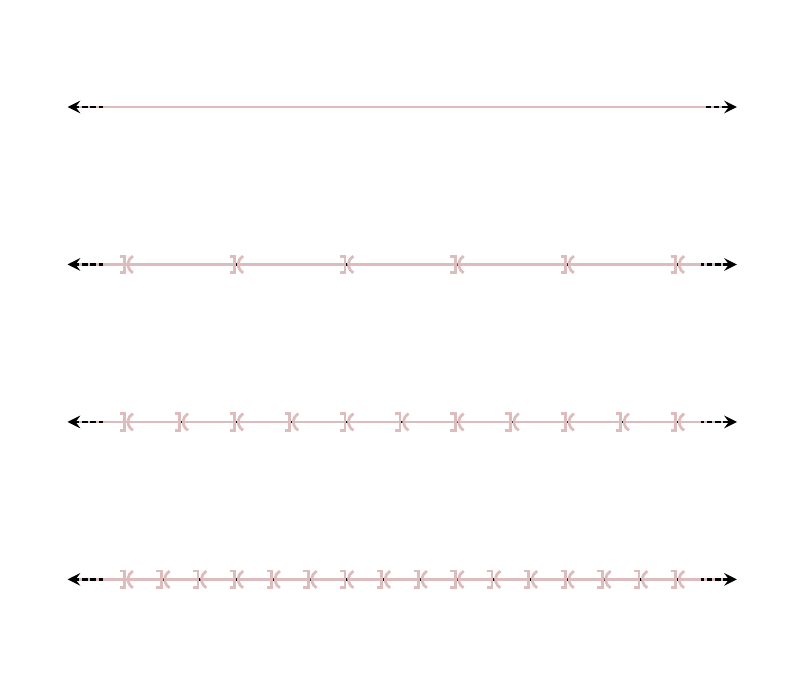
\begin{tikzpicture}[scale=1]
  
   \draw[white] (-4.75, -5) rectangle (4.75, 3);
  
  \begin{scope}[shift={(0, 0)}]
    \pgfmathsetmacro{\delta}{0.01}
    
    \pgfmathsetmacro{\y}{2}
    \draw[<->, >=stealth, line width=1] (-4.25, \y) -- (+4.25, \y);
      
    \draw[light, dotted, line width=1] (-4.1, \y) -- ({-4 + 0.5 - \delta}, \y);
    \draw[light, line width=1] ({-4 + 0.2}, \y) -- ({4 - 0.15}, \y);  
    \draw[light, dotted, line width=1] ({4 - 0.5}, \y) -- (4.1, \y);
    
    \foreach [count=\m] \N in {5, 10, 15} {
      \pgfmathsetmacro{\l}{7 / \N}
      \pgfmathsetmacro{\y}{2 * (1 - \m)}
      
      \draw[<->, >=stealth, line width=1] (-4.25, \y) -- (+4.25, \y);
      
      \draw[arrows={-Bracket[sharp]}, light, dotted, line width=1] (-4.1, \y) -- ({-4 + 0.5 - \delta}, \y);
      \draw[light, line width=1] ({-4 + 0.2}, \y) -- ({-4 + 0.5}, \y); 
      
      \foreach \n in {1, 2, ..., \N} {
        \pgfmathsetmacro{\x}{-3.5 + (\n - 1) * \l}
        \draw[arrows={Parenthesis[sharp]-Bracket[sharp]}, light, line width=1] ({\x}, \y) -- ({\x + \l - \delta}, \y);
      }
      
      \draw[arrows={Parenthesis[sharp]-}, light, dotted, line width=1] ({4 - 0.5}, \y) -- (4.1, \y);
      \draw[light, line width=1] ({4 - 0.2}, \y) -- ({4 - 0.5}, \y); 
    }
  \end{scope}
  
\end{tikzpicture}

\end{document}  